\documentclass[times,specification,annotation]{itmo-student-thesis}

%% Опции пакета:
%% - specification - если есть, генерируется задание, иначе не генерируется
%% - annotation - если есть, генерируется аннотация, иначе не генерируется
%% - times - делает все шрифтом Times New Roman, собирается с помощью xelatex
%% - pscyr - делает все шрифтом Times New Roman, требует пакета pscyr.

%% Делает запятую в формулах более интеллектуальной, например:
%% $1,5x$ будет читаться как полтора икса, а не один запятая пять иксов.
%% Однако если написать $1, 5x$, то все будет как прежде.
\usepackage{icomma}

%% Один из пакетов, позволяющий делать таблицы на всю ширину текста.
\usepackage{tabularx}

%% Данные пакеты необязательны к использованию в бакалаврских/магистерских
%% Они нужны для иллюстративных целей
%% Начало
\usepackage{tikz}
\usetikzlibrary{arrows,automata,positioning}
\usepackage{filecontents}
\begin{filecontents}{bachelor-thesis.bib}
@online{ doerr-doerr-lambda-lambda-self-adjustment-arxiv,
    year        = {2015},
    title       = {Optimal Parameter Choices Through Self-Adjustment: Applying the 1/5-th Rule in
                   Discrete Settings},
    author      = {Benjamin Doerr and Carola Doerr},
    url         = {http://arxiv.org/abs/1504.03212},
    year        = {2015},
    langid      = {english}
}

@inproceedings{ example-english,
    year        = {2015},
    booktitle   = {Proceedings of IEEE Congress on Evolutionary Computation},
    author      = {Maxim Buzdalov and Anatoly Shalyto},
    title       = {Hard Test Generation for Augmenting Path Maximum Flow 
                   Algorithms using Genetic Algorithms: Revisited},
    pages       = {2121-2128},
    langid      = {english}
}

@article{ example-russian,
    author      = {Максим Викторович Буздалов},
    title       = {Генерация тестов для олимпиадных задач по программированию 
                   с использованием генетических алгоритмов},
    journal     = {Научно-технический вестник {СПбГУ} {ИТМО}},
    number      = {2(72)},
    year        = {2011},
    pages       = {72-77},
    langid      = {russian}
}

@article{ unrestricted-jump-evco,
    author      = {Maxim Buzdalov and Benjamin Doerr and Mikhail Kever},
    title       = {The Unrestricted Black-Box Complexity of Jump Functions},
    journal     = {Evolutionary Computation},
    year        = {2016},
    note        = {Accepted for publication},
    langid      = {english}
}

@book{ bellman,
    author      = {R. E. Bellman},
    title       = {Dynamic Programming},
    address     = {Princeton, NJ},
    publisher   = {Princeton University Press},
    numpages    = {342},
    pagetotal   = {342},
    year        = {1957},
    langid      = {english}
}

@article { state-merging-dfa,
    author      = {Bernard Lambeau and Christophe Damas and Pierre Dupont},
    title       = {State-Merging DFA Induction Algorightms with Mandatory Merge Constraints},
    pages       = {139-153},
    journal     = {Lecture Notes in Computer Science},
    year        = {2008},
    langid      = {english},
    url         = {https://www.info.ucl.ac.be/~pdupont/pdupont/pdf/icgi08.pdf}
}

@article { rti,
    author      = {Sicco Verwer and Mathijs de Weerdt and Cees Witteveen},
    title       = {Efficiently identifying deterministic real-time automatafrom labeled data},
    pages       = {295-333},
    journal     = {Springer},
    year        = {2010},
    langid      = {english},
    url         = {https://link.springer.com/article/10.1007/s10994-011-5265-4}
}

@article { timed-k-tail,
    author      = {Fabrizio Pastore and Daniela Micucci and Leonardo Mariani},
    title       = {Timed k-Tail: Automatic Inference of Timed Automata},
    numpages    = {11},
    pagetotal   = {11},
    year        = {2017},
    langid      = {english},
    url         = {https://arxiv.org/pdf/1705.08399.pdf}
}

@article { k-tail,
    author      = {Alan Biermann and Jerome Feldman},
    title       = {On the Synthesis of Finite-State Machines from Samples of Their Behavior},
    pages       = {592-597},
    journal     = {IEEE Transactions on Computers},
    year        = {1972},
    langid      = {english},
    url         = {https://www.researchgate.net/publication/224483188_On_the_Synthesis_of_Finite-State_Machines_from_Samples_of_Their_Behavior}
}
\end{filecontents}
%% Конец

%% Указываем файл с библиографией.
\addbibresource{bachelor-thesis.bib}

\begin{document}

\studygroup{M3439}
\title{Пример оформления ВКР бакалавра}
\author{Буздалов Максим Викторович}{Буздалов М.В.}
\supervisor{Шалыто Анатолий Абрамович}{Шалыто А.А.}{проф., д.т.н.}{главный научный сотрудник Университета ИТМО}
\publishyear{2019}
%% Дата выдачи задания. Можно не указывать, тогда надо будет заполнить от руки.
\startdate{01}{сентября}{2018}
%% Срок сдачи студентом работы. Можно не указывать, тогда надо будет заполнить от руки.
\finishdate{31}{мая}{2019}
%% Дата защиты. Можно не указывать, тогда надо будет заполнить от руки.
\defencedate{15}{июня}{2019}

\addconsultant{Белашенков Н.Р.}{канд. физ.-мат. наук, без звания}
\addconsultant{Беззубик В.В.}{без степени, без звания}

\secretary{Павлова О.Н.}

%% Задание
%%% Техническое задание и исходные данные к работе
\technicalspec{Требуется разработать стилевой файл для системы \LaTeX, позволяющий оформлять бакалаврские работы и магистерские диссертации
на кафедре компьютерных технологий Университета ИТМО. Стилевой файл должен генерировать титульную страницу пояснительной записки,
задание, аннотацию и содержательную часть пояснительной записк. Первые три документа должны максимально близко соответствовать шаблонам документов,
принятым в настоящий момент на кафедре, в то время как содержательная часть должна максимально близко соответствовать ГОСТ~7.0.11-2011
на диссертацию.}

%%% Содержание выпускной квалификационной работы (перечень подлежащих разработке вопросов)
\plannedcontents{Пояснительная записка должна демонстрировать использование наиболее типичных конструкций, возникающих при составлении
пояснительной записки (перечисления, рисунки, таблицы, листинги, псевдокод), при этом должна быть составлена так, что демонстрируется
корректность работы стилевого файла. В частности, записка должна содержать не менее двух приложений (для демонстрации нумерации рисунков и таблиц
по приложениям согласно ГОСТ) и не менее десяти элементов нумерованного перечисления первого уровня вложенности (для демонстрации корректности
используемого при нумерации набора русских букв).}

%%% Исходные материалы и пособия 
\plannedsources{\begin{enumerate}
    \item ГОСТ~7.0.11-2011 <<Диссертация и автореферат диссертации>>;
    \item С.М. Львовский. Набор и верстка в системе \LaTeX;
    \item предыдущий комплект стилевых файлов, использовавшийся на кафедре компьютерных технологий.
\end{enumerate}}

%%% Цель исследования
\researchaim{Разработка удобного стилевого файла \LaTeX
             для бакалавров и магистров кафедры компьютерных технологий.}

%%% Задачи, решаемые в ВКР
\researchtargets{\begin{enumerate}
    \item обеспечение соответствия титульной страницы, задания и аннотации шаблонам, принятым в настоящее время на кафедре;
    \item обеспечение соответствия содержательной части пояснительной записки требованиям ГОСТ~7.0.11-2011 <<Диссертация и автореферат диссертации>>;
    \item обеспечение относительного удобства в использовании~--- указание данных об авторе и научном руководителе один раз и в одном месте, автоматический подсчет числа тех или иных источников.
\end{enumerate}}

%%% Использование современных пакетов компьютерных программ и технологий
\addadvancedsoftware{Пакет \texttt{tabularx} для чуть более продвинутых таблиц}{\ref{sec:tables}, Приложения~\ref{sec:app:1}, \ref{sec:app:2}}
\addadvancedsoftware{Пакет \texttt{biblatex} и программное средство \texttt{biber}}{Список использованных источников}

%%% Краткая характеристика полученных результатов 
\researchsummary{Получился, надо сказать, практически неплохой стилевик. В 2015--2018 годах
его уже использовали некоторые бакалавры и магистры. Надеюсь на продолжение.}

%%% Гранты, полученные при выполнении работы 
\researchfunding{Автор разрабатывал этот стилевик исключительно за свой счет и на
добровольных началах. Однако значительная его часть была бы невозможна, если бы
автор не написал в свое время кандидатскую диссертацию в \LaTeX,
а также не отвечал за формирование кучи научно-технических отчетов по гранту,
известному как <<5-в-100>>, что происходило при государственной финансовой поддержке
ведущих университетов Российской Федерации (субсидия 074-U01).}

%%% Наличие публикаций и выступлений на конференциях по теме выпускной работы
\researchpublications{По теме этой работы я (к счастью!) ничего не публиковал.
\begin{refsection}
Однако покажу, как можно ссылаться на свои публикации из списка литературы:
\nocite{example-english, example-russian}
\printannobibliography
\end{refsection}
}

%% Эта команда генерирует титульный лист и аннотацию.
\maketitle{Бакалавр}

%% Оглавление
\tableofcontents

%% Макрос для введения. Совместим со старым стилевиком.
\startprefacepage

Пока что не знаю, что здесь написать. Скорее всего, никогда не узнаю.

%% Начало содержательной части.
\chapter{Постановка задачи}

В настоящее время широко распространены системы реального времени. 
Остро стоит вопрос построения модели данной системы реального времени. 
На практике зачастую сложно создать модель по имеющейся системе. 
Гораздо более легким подходом оказывается генерация моделей по примерам их поведения. 
Одной из наиболее востребованных и изученных моделей является Детерминированный Конечный Автомат (ДКА). 
Данный вид моделей хорошо изучен в теории формальных языков и для него разработано множество алгоритмов.

Примеры поведения моделей обычно представляют собой список событий, которые произошли с системой, аннотированные временем, которое прошло после предыдущего события.
Для систем реального времени конкретно данный вид моделей подходит плохо, так как ДКА практически никак не учитывает время. 
Тем не менее, в данную модель возможно внести время прямолинейным способом, если ввести некоторое нулевое событие, которое описывает атомарную единицу времени. 
Данный подход плох тем, что теперь, чтобы адаптировать примеры поведения в данного ДКА, необходимо перевести все задержки во времени в унарную систему счисления, что приведет к экспоненциальному росту длины самих примеров и, как следствие, индуциованной по данным примерам модели.
Но существует модель, очень близкая по строению к существующей модели Детерминированного Конечного Автомата, хорошо обрабатывающая время, как раз нацеленная на использование в качестве модели для систем реального времени.

\section{Термины и понятия}
В данном разделе будут приведены определения терминов, которые будут использоваться в следующих главах, а также основные результаты о временных автоматах.

\begin{definition}
  Временное ограничение $g$ -- предикат на таймерах. Его можно получить одним из трех способов:
  \begin{itemize}
    \item $g := c \leq x$
    \item $g := c \geq x$
    \item $g := g_1 \land g_2$
  \end{itemize}
  где $g$ -- временное ограничение, $c \in C$ -- таймер, $x \in \mathbb{N}$ -- граница ограничения
\end{definition}

\begin{definition}
  Временной автомат $\mathcal{A}$ -- кортеж $\langle \Sigma, Q, q_0, C, \Delta, F \rangle$, где
  \begin{itemize}
    \item $\Sigma$ -- алфавит(множество символов) автомата,
    \item $Q$ -- конечное множество состояний,
    \item $q_0 \in Q$ -- начальное состояние автомата,
    \item $C$ -- конечное множество таймеров,
    \item $F \subseteq Q$ -- множество принимающих состояний.
    \item $\Delta$ -- конечное множество переходов, где переход -- это кортеж $\langle q_1, q_2, a, g, R \rangle$, где
    \begin{itemize}
      \item $q_1, q_2 \in Q$ - начальное и конечное состояние, которые соединяет данный переход,
      \item $a \in \Sigma$ - символ, по которому осуществляется переход,
      \item $g$ - временные ограничения на таймерах,
      \item $R \in 2^{C}$ - таймеры, которые нужно сбросить после перехода по $\delta$. 
    \end{itemize}
  \end{itemize}
\end{definition}

\begin{example}
  На рисунке~\ref{time_automaton} приведен пример временного автомата. 
  Состояние $q_3$ является принимающим, все же остальные принимающими не являются. 
  Начальным состоянием временного автомата является $q_0$. 
  Из него исходит одно ребро в состояние $q_1$ с символом перехода $a$. 
  После перехода по данному ребру таймер $x$ сбрасывается. 
  Из состояния $q_1$ тоже исходит ребро в состояние $q_2$ с символом перехода $b$, но уже с ограничением на таймер $x$.
  Чтобы пройти по данному ребру таймер $x$ должен быть меньше единицы.
  Лучше всего использование таймеров демонстрируют два перехода из состояния $q_2$, так как из-за таймеров, чтобы пройти в состояние $q_3$, необходимо будет 20 раз пройти по петле в то же состояние $q_2$.
\end{example}

\begin{figure}[!h]
\caption{Пример временного автомата}\label{time_automaton}
\centering
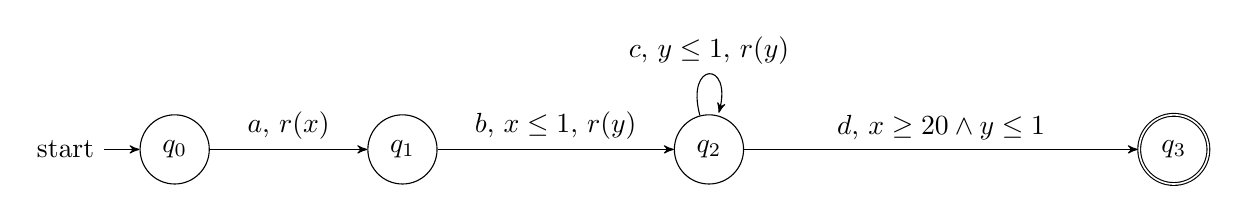
\begin{tikzpicture}[>=stealth']
  \node[state, initial] (q0) {$q_0$};
  \node[state] (q1) [right=2cm of q0] {$q_1$};
  \node[state] (q2) [right=3cm of q1] {$q_2$};
  \node[state, accepting] (q3) [right=5cm of q2] {$q_3$};
  \path[->]
  (q0) edge node[anchor=center, above] {$a$, $r(x)$} (q1)
  (q1) edge node[anchor=center, above] {$b$, $x \leq 1$, $r(y)$} (q2)
  (q2) edge [loop above] node[anchor=center, above] {$c$, $y \leq 1$, $r(y)$} ()
       edge node[anchor=center, above] {$d$, $x \geq 20 \land y \leq 1$} (q3);
\end{tikzpicture}
\end{figure}

\begin{definition}
  Трассировка $\tau$ -- последовательность пар $\{\left( a, t \right)\}$, 
  где $t \in \mathbb{N}$ -- задержка между предыдущим и текущим событиями, $a \in \Sigma$ -- символ перехода.
\end{definition}

\begin{definition}
  Значение $\nu(x)$ таймера $x \in C$ -- функция из таймера $x$ в $\mathbb{N}$
\end{definition}

\begin{definition}
  Путь во временном автомате по трассировке $\{\left( a_i, d_i \right)\}$ -- последовательность из пар $\{\left( q_i, \nu_i \right)\}$, таких что $q_i \in Q$ -- состояние на шаге $i$, $\nu_i$ -- значения таймеров на шаге $i$
  и для которых выполняются следующие ограничения:
  \begin{itemize}
    \item $q_{2i} = q_{2i+1}$
    \item $\forall x \in C: \nu_{2i+1}(x) - \nu_{2i}(x) = d_i$
    \item $\exists! \langle q^1, q^2, a, g, R \rangle \in \Delta$: 
      \begin{itemize}
	\item $q_{2i+1} = q^1$
	\item $q_{2i+2} = q^2$
        \item $\forall x \in R: \nu_{2i+2}(x) = 0$
	\item $\forall x \not\in R: \nu_{2i+2}(x) = \nu_{2i+1}(x)$
	\item $\forall x \in C: \nu_{2i+1}(x)$ удовлетворяет $g$
      \end{itemize}
  \end{itemize}
\end{definition}

Другими словами, в пути во временном автомате каждая пара из состояния и значений таймеров с четным номером отличается от предыдущей изменением состояния автомата, а также, возможно, сбрасыванием некоторого количества таймеров, каждая же пара с нечетным индексом отличается от предыдущей только увеличением значений таймеров.

\begin{definition}
  Языком $\mathcal{L}(\mathcal{A})$ временного автомата $\mathcal{A}$ назовем множество всех принимаемых трассировок.
\end{definition}

\begin{definition}
  Класс автоматов $\mathbb{K}$ называется достижимым за полином, если существует полином $p$ такой, что для любых
  $\mathcal{A} \in \mathbb{K}, q \in Q_{\mathcal{A}}$ существует трассировка $\tau$ такая, что порожденный ей путь заканчивается в $q$ и $|\tau| < p(|\mathcal{A}|)$.
\end{definition}

\section{Известные результаты}
\begin{lemma}
  Класс временных автоматов не является достижимым за полином.
  \label{unreachable_lemma}
\end{lemma}

Лемма~\ref{unreachable_lemma} фактически утверждает, что, чтобы однозначно правильно синтезировать автомат по примерам, необходимо в качество примеров иметь так же пример экспоненциальной длины от размера временного автомата.

\begin{definition}
  Класс автоматов $\mathbb{K}$ называется различимым за полином, если существует полином $p$ такой, что для любых
  $\mathcal{A}, \mathcal{A'} \in \mathbb{K}, \mathcal{L}(\mathcal{A}) \neq \mathcal{L}(\mathcal{A'})$ существует трассировка $\tau$ такая, что 
  $\tau \in \mathcal{L}(\mathcal{A}) \Delta \mathcal{L}(\mathcal{A'})$ и $|\tau| < p(|\mathcal{A}| + |\mathcal{A'}|)$
\end{definition}

\begin{lemma}
  Класс временных автоматов не различим за полином.
  \label{distinguishability_lemma}
\end{lemma}

\begin{definition}
    Характеристическим множеством языка $\mathcal{L}_t$ для алгоритма $A$ называется множество трассировок $S_{cs} = \{S_{cs+}, S_{cs-}\}$, где
  $S_{cs+} \subseteq \mathcal{L}_t$, $S_{cs-} \subseteq \mathcal{L}_t^c$, такое, что 
  для любого $S \supseteq S_{cs}, S_+ \subseteq \mathcal{L}_t, S_- \subseteq \mathcal{L}_t^c$ алгоритм $A$ на вход $S$ вернет автомат $\mathcal{A}$ такой, что $\mathcal{L}(\mathcal{A}) = \mathcal{L}_t$.
\end{definition}

\begin{definition}
    Класс автоматов $\mathbb{K}$ является эффективно синтезируемым в пределе, если существуют полиномы $p, q$ и алгоритм $A$ такие, что
  \begin{itemize}
    \item Время работы алгоритма на входе $S$ ограничено сверху $p(\mathop{\sum}\limits_{\tau \in S}|\tau|)$
    \item Для любого языка $\mathcal{A} \in \mathbb{K}$ существует $S_{cs} $ -- характеристическое множество языка $\mathcal{A}$ для алгоритма $A$ такой, что $\mathop{\sum}\limits_{\tau \in S_{cs}}|\tau| < q(|\mathcal{A}|)$
  \end{itemize}
\end{definition}

\begin{theorem}
    Класс временных автоматов не является эффективно синтезируемым
  \label{efficient_synthesis_theorem}
\end{theorem}

Доказаны также некоторые послабления данной теоремы.

\begin{theorem}
  Если $coNP \neq PSPACE$, то временной автомат не может быть эффективно синтезирован.
  \label{coNPneqPSPACE_lemma}
\end{theorem}

\begin{theorem}
  Если $NP \neq PSPACE$, то временной автомат не может быть эффективно синтезирован.
  \label{NPneqPSPACE_lemma}
\end{theorem}

Хоть и было доказано, что класс временных автоматов в целом не является эффективно синтезируемым, из него возможно выделить подкласс временных автоматов, который бы являлся эффективно синтезируемым.
Приведем формулировку теоремы, которая немного проясняет ситуацию с временными автоматами.

\begin{theorem}
  Класс временных автоматов, в котором используется два или больше таймеров не может быть эффективно синтезирован.
  \label{two_or_more_timers_lemma}
\end{theorem}

Таким образом, возможно стоит данный подкласс во временных автоматах, которые могут использовать всего таймер? 
На самом деле в статье (должен быть реф) были доказаны следующие факты:

\begin{lemma}
  Класс временных автоматов с одним таймером является полиномиально достижимым.
  \label{reachability_1_lemma}
\end{lemma}

\begin{lemma}
  Класс временных автоматов с одним таймером является полиномиально различимым.
  \label{distinguishability_1_lemma}
\end{lemma}

\begin{theorem}
  Класс временных автоматов с одним таймером является эффективно синтезируемым.
  \label{efficient_synthesis_1_theorem}
\end{theorem}

\begin{definition}
  Автомат реального времени -- временной автомат такой, что $C = \{c_0\}, R_{\delta} = \{c_0\}$ для любого перехода $\delta \in \Delta$.
  \label{rti}
\end{definition}

В качестве доказательства теоремы~\ref{efficient_synthesis_1_theorem} авторы статьи (должен быть реф) предоставили интересный алгоритм, который хотелось бы разобрать.

\section{Эффективный синтез временного автомата с одним таймером с помощью алгоритма ID-DTA-1}

В алгоритме временной автомат строится итеративно. Алгоритм выполняется, пока существует трассировка, 
некоторый префикс которой заканчивается в состоянии $q$ и из этого состояния не существует перехода $\langle q, q', a, g, r \rangle$ по символу $a$, удовлетворяя ограничения $g$.
На каждой итерации алгоритм перебирает текущие состояния автомата и выбирает минимальное значение таймера $v_{min}$, с которым можно добраться до текущего состояния,
а также максимальное значение таймера $c'$, для которого не существует перехода по символу $a$, удовлетворяя ограничения $g$. Если $v_{min} \leq c'$, то значит мы не можем перейти по
символу $a$ для текущей трассировки с таймером $v_{min}$. Нужно выбрать нижнюю границу нового перехода. Ее выбираем минимальной, после добавления перехода с такой нижней границей,
можно корректно достроить автомат. В качестве возможной нижней границы попробуем подставить всевозможные значения таймеров, которые можно получить, проходя по существующим трассировкам.
Корректно достроить автомат можно, если не существует принимающейся и отвергающейся трассировок, префиксы которых приводят в одно и то же состояние,
далее идет переход по одинаковому символу с ожиданиями, выравнивающими значения таймеров на следующем состоянии, и далее суффиксы этих трассировок совпадают. Соответственно, алгоритм
выбирает минимальную границу из ситуации, когда на данном ребре есть сброс таймера и когда его нет. Осталось выбрать конечное состояние для данного ребра. Выбираем первое состояние,
при проведении данного ребра в которое автомат до сих пор сможет корректно достроить автомат. Если такого состояния не существует, добавляем новую вершину и проводим ребро в него.
Следующая вершина будет принимающей в случае, если существует трассировка $\tau$, которая заканачивается в нем и $\tau \in S_+$.

\section{Эффективный синтез автомата реального времени с помощью алгоритмы RTI}

Данный алгоритм основан на адаптации текущего state-of-the-art алгоритма синтеза конечных детерминированных автоматов EDSM~\cite{state-merging-dfa}. 
Данный алгоритм начинает синтез автомата с построения префиксного дерева трассировок. Данное префиксное дерево будет выступать в качестве первоначального автомата.
Далее алгоритм пытается находить состояния, которые, как он предполагает, являются одинаковыми в минимальном конечном автомате и сливает их.

EDSM синтезирует автомат в так называемой красно-синей среде. Данная среда представляет собой ни что иное, как разделение множества всех состояний на
множество красных состояний, которые являются уже просмотренными, множество синих состояний, которые сейчас рассматриваются и множество непокрашенных
состояний, которые на данном шаге никак не рассматриваются. Красные состояния получаются окаймлены синими, то есть
для каждого синего состояния на текущем шаге есть красное состояние с ребром, которое ведет в данное синее. 

На данном шаге выбирается один из двух вариантов: слить два состояния, либо покрасить синее состояние в красное. Слить можно либо два синих состояния,
либо красное состояние с синим. Предолагается, что между двумя красными состояниями переходы никаким образом поменяться не могут. При слиянии двух состояний 
множество переходов, выходящих из этих двух состояний, объединяются. Но тогда получившийся автомат может оказаться уже недетерминированным: из новой вершины,
слитой из двух, может оказаться два ребра с переходом по одному и тому же символу. Данная проблема решается слиянием вершин, в которые ведут данные ребра. Тогда
два ребра, из-за которых образуется недетерминизм сливаются так же в одно. Но не всегда два состояния можно слить, иначе бы всегда получался автомат из одной вершины.
Предикатом на возможность слияния двух вершин будет то, что сливаемые вершины не должны быть разными по принятию трассировок (одна -- принимающей, вторая -- отвергающей), а также, 
если произошла ситуация недетерминизма, все потомки, которые необходимо слить, так же должны удовлетворять предикату на возможность слияния.
Возможна так же ситуация, что на текущем шаге лучше покрасить синию вершину в красную, что сливать вершины.

Нужно упомянуть, что синтез автомата в красно-синей среде не ограничивает в возможности найти корректный минимальный автомат, ведь в некоторый момент каждая из вершин становится
синей и именно в этот момент необходимо корректно определить, нужно ли её слить с какой-то посещенной вершиной или же наоборот пропустить, чтобы потом слить какой-нибудь
ещё непосещенной вершиной. Таким образом, размер автомата, который получится в конце, определяется стратегией, которую выбирают при синтезе автомата.
Так как абсолютно правильную стратегию сливаний и перекрасок выбрать сложно, из-за того, что задача синтеза минимального конечного детерминированного автомата по трассировкам это
NP-полная задача, то для этого применяют эвристики. В алгоритме EDSM используется используется эвристика для оценки правильности некоторой операции. Эта оценка является просто натуральным
числом. Тогда на текущей итерации оценивают правильность всевозможных слияний, всевозможных покрасок и применяют ту, для которой оценка является наивысшей величиной среди остальных.
В качестве оценки обычно выступает оценка качества автомата, который получается после применения данной операции.
В EDSM обычно применяют следующую эвристическую оценку:

\begin{equation}
  pure = \#pos + \#neg
  \label{heur_1}
\end{equation}

В эвристике~\ref{heur_1} $\#pos$, $\#neg$ - количество слитых вершин, которые обе были принимающие и отвергающие соответственно. При равенстве нескольких наилучших оценок выбирают сначала
слияние, а затем покраску. Иными словами, с данной эвристикой у покраски всегда оценка правильности равна ноль. Таким образом, она будет произведена только в случае, 
если больше не осталось вершин, которые можно было бы слить. В качестве вершины для покраски можно выбирать любую.

Авторы алгоритма RTI~\cite{rti} адаптировали алгоритм EDSM, чтобы он мог использовать время. Авторам статьи для этого пришлось добавить в исходный алгоритм еще одну операцию -- разделение.
Изначально строится такое же префиксное дерево, как и в EDSM, без учета временных составляющих трассировок, и каждому переходу в префиксном дереве выставляется максимальные ограничения на переход.
При таком подходе некоторые трассировки могли попасть в префиксном дереве в одну и ту же вершину, хотя, возможно, одна из них являлася принимаемой, а другая -- отклоняемой. Таким образом, временной
автомат изначально не всегда является консистентным. Но в конце алгоритма он должен быть таковым. Так как, как и алгоритм EDSM, RTI работает в красно-синей среде, и между красными состояниями
переходы не меняются, то необходимо, чтобы на каждом шаге красная часть автомата была консистентной, а также чтобы остальную часть автомата можно было превратить в консистентную
операциями слияния, разделения и перекраски. Изначальную неконсистентность исправляют операциями разделения. Возможно провести разделение только тех ребер, которые ведут из красных состояний в синие. 
При разделении ребра крайне нежелательно, чтобы два новых ребра вели в то же самое состояние, так как в таком случае это никак не избавит от неконсистентности.
Решается эта проблема глубоким копированием всего, куда ведёт резделяемое ребро. Это можно сделать потому что, всё, до чего можно добраться, проходя по разделяемому ребру, это либо синее, либо
непокрашенное состояние. То есть, на самом деле, это префиксное дерево из непокрашенных вершин. Поэтому из него нет ребер в красные состояния, и данную часть автомата можно без опасений скопировать.
Разделение ещё применяют в качестве вспомогательной операции при слиянии. Заметим, что так как разделение можно применить только на ребрах из красных состояний в синие, ребра выходящие из синих
вершин являются нетронутыми, а значит имеющими изначальные максимальные ограничения на переход. Поэтому перед тем как слить синее состояние с красным алгоритм RTI разбивает ребра, 
выходящие из синего состояния в тех же пропорциях, в которых находятся ребра, выходящие из красной вершины. В данном случае так же применяется глубокое копирование выходящих префиксных деревьев.
Проверка на то, что автомат можно достроить до консистентного точно такая же, как и в EDSM алгоритме (предикат на возможность слияния).

Аналогично, нужно упомянуть, что добавленная операция разделения не повлияет на возможность нахождения минимального временного автомата: необходимо в момент, когда состояние, из которого
выходят ребро, стало красным, а значит состояние, в которое входит, стало синим, провести правильное количество разделений данного ребра в корректных местах. Но на практике у операции
разделения куда меньший приоритет по сравнению с операцией слияния, так как при слиянии как раз и произойдёт, скорее всего, самое правильное разбиение ребер. 

В алгоритме RTI точно так же применяется некоторое множество эвристических оценок. Первая из них -- это эвристика \ref{heur_1}, заимствованная из алгоритма EDSM. 
В качестве оценки правильности операций разделения тоже можно выбрать ноль. При равенстве нескольких наилучших оценок операций приоритет отдается сначала слиянию, затем разделению, а затем покраске.

Следующая эвристика -- это подправленная эвристика \ref{heur_1}. В отличие в неё в данной эвристике так же учитывается количество новых неконсистентных состояний.

\begin{equation}
  consistent = \#pos + \#neg - \#posneg
  \label{heur_2}
\end{equation}

В эвристике~\ref{heur_2} $\#pos$, $\#neg$ -- так же количество слитых вершин, которые обе принимающие или отвергающие, $\#posneg$ -- количество вершин, которые являются неконсистентными, то есть
существуют минимум две трассировки, одна из которых принимаемая, другая отвергаемая, которые заканчиваются в данном состоянии.

Следующая эвристика уже не является столь простой, но она по сути является расширением предыдущей эвристики, а именно расширяется понимание $\#posneg$. Ведь интуитивно кажется, что
если трассировки, ведущие в неконсистентное состояние имеют большие разбросы по времени, то их легко разделить, и они не должны вносить сильный отрицательный вклад. А вот такие же строки,
которые имеют практически одинаковые времена на пути к неконсистентному состоянию, должны давать наоборот большой отрицательный вклад.
Таким образом, в этой эвристике особый упор отдается времени. Для каждых двух путей до листьев в префиксном дереве (временных строк), 
для которых одинаковы последовательности событий без времен, считается их похожесть. Так как их последовательности событий без времен одинаковы, они заканчиваются в одном и том же листе 
префиксного дерева. Похожесть двух строк определяется как вероятность того, что данные строки можно разделить, разделив равновероятно одно из ребер на пути от корня до листа, выбрав в качестве
времени для разделения временного ограничения равновероятно любую его точку. Эвристика выглядит следующим образом:

\begin{equation}
  \begin{split}
    impact = \mathop{\sum}\limits_{q \in Q_r}pure(q) - \mathop{\sum}\limits_{\tau \in \Delta_b}max\{impact(\tau, \tau') | \tau \in S^\delta_+ \land \tau' \in S^\delta_-\}& \\
						     + \mathop{\sum}\limits_{\tau \in \Delta_b}max\{impact(\tau, \tau') | \tau \in S^\delta_+ \land \tau' \in S^\delta_+\}& \\ 
						     + \mathop{\sum}\limits_{\tau \in \Delta_b}max\{impact(\tau, \tau') | \tau \in S^\delta_- \land \tau' \in S^\delta_-\}&
  \end{split}
  \label{heur_3}
\end{equation}

В эвристике~\ref{heur_3} $impact(\tau, \tau')$ -- похожесть двух временных строк $\tau$ и $\tau'$, $pure(q)$ -- эвритическая оценка EDSM только для вершины $q$, 
$S^\delta_+$, $S^\delta_-$ -- принимаемые и отвергаемые трассировки соответственно, которые в своем пути по текущему автомату проходят по ребру $\delta$.

Последняя эвристическая оценка тоже добавляет в изначальную оценку EDSM влияние неконсистентных вершин. В данном случае пытаются учесть величину того,
сколько потребуется разделений, чтобы избавить непокрашенные префиксные деревья от неконсистентных вершин. Так как точное количество посчитать сложно из-за $NP$-трудности
данной задачи, применяется некоторый жадный алгоритм. Эвристическая оценка имеет следующий вид:

\begin{equation}
  splits = \mathop{\sum}\limits_{q \in Q}max(pure(q) - \#split(q), 0)
  \label{heur_4}
\end{equation}

В эвристике~\ref{heur_4} $\#splits(q)$ -- приблизительное количество разделений, необходимых для избавления от неконсистентных состояний в префиксном дереве, выходящем из вершины $q \in Q$.

При тестировании лучше всего себя показали эвристические оценки \ref{heur_2} и \ref{heur_4}.

\section{Подход к синтезу в алгоритме Timed-k-Tail}

Данный алгоритм Timed-k-Tail\cite{timed-k-tail} является адаптацией алгоритма k-Tail\cite{k-tail}, применяемого для синтеза детерминированных конечных автоматов без негативных примеров поведения. 
Алгоритм Timed-k-Tail нацеливается на генерацию автомата, хорошо описывающего поведение реальных программ. Предпологается, что есть некоторая эталонная программа, 
все трассировки которой являются корректными. Нужно построить некоторый автомат, имея только корректные трассировки, полученные при запусках данной программы, чтобы
можно было, в частности, валидировать корректность работы аналогичных программ. Трассировки для данного алгоритма тоже подойдут не любые.
События для данных трассировок делятся на два вида: начало некоторой функции и конец некоторой функции. Трассировка должна быть правильной скобочной последовательностью, если назначить 
начало функций в качестве открывающейся скобки, а конец в качестве закрывающейся скобки, причем у разных функций должны быть разные скобки.
Алгоритм делится на несколько стадий.

Первая стадия данного алгоритма -- нормализация. На вход изначально потупает некоторое множество трассировок выполнения реальной программы. Первое, что происходит в алгоритме,
так это изменяются трассировки таким образом, чтобы время старта для каждой трассировки было одинаковым: обычно от каждого времени в трассировке отнимают время первого события
в данной трассировке, таким образом выходит, что первое событие каждой трассировки стартует в момент времени ноль. Но все задержки времени между любой парой событий в трассировке
сохраняются неизменными. 

Вторая стадия -- построение по трассировкам префиксного дерева. В данном алгоритме используется огромное количество таймеров, чтобы замерять задержки между началом функции в некоторый
момент времени и её концом. Также будет существовать один нулевой (глобальный) таймер $t$, который нельзя будет сбрасывать. Видоизменим трассировки. 
Во-первых, каждая трассировка теперь будет аннотироваться не временем, а ограничениями и множеством таймеров для сброса. В качестве первого ограничения для каждого события $j$ в трассировке $i$
добавим $t = time_{i, j}$, где $time_{i, j}$ -- момент времени, в который произошло событие $j$ в трассировке $i$. Далее для каждого события начала функции добавим во множество сброса новый
таймер. Пусть в трассировке $i$ для события $j$ этот таймер будет иметь номер $с$. Тогда в трассировке $i$ нужно найти событие конца данной функции. Пусть оно по номеру равно $k$. И в его
аннотацию добавить ещё одно ограничение $c = time_{i, k} - time_{i, j}$. Таким образом замеряется время работы каждого запуска какой-либо функции. Последнее, что нужно сделать,
первому событию в каждой из трассировок добавить во множество сброса таймер $t$, таким образом позволяя не думать о том, какими таймеры могут быть в корне будущего префиксного дерева, все они всё равно
в будущем будут сброшены. И только после данных операций по видоизмененным трассировкам нужно построить префиксное дерево.

Третья стадия -- слияние состояний. На текущем этапе нужно выбрать величину $k$, присутствующую в названии данного алгоритма. Идея, которая главенствует на данной стадии синтеза автомата,
гласит, что ``скорее-всего'' система находится в одном и том же состоянии, если, как минимум, первые $k$ событий, исходящие из двух состояний, совпадают. Но нужно также разобраться с ребрами, которые
получаются при слиянии двух состояний. Алгоритм предписывает реберам, выходящим из сливаемых состояний, с одинаковым переходным символом так же слиться, при этом объединяя множества сбросов и
множество ограничений. 

Четвертая стадия -- улучшение таймеров. К текущему моменту у автомата может возникнуть много таймеров, которые мериют одно и то же из-за того, что на предыдущей стадии произошло слияние состояний.
На данном этапе нужно избавиться от таких таймеров. Пара таймеров мериет одно и то же, если каждый из них сбрасывается и проверяется на одних и тех же переходах. Находим все таймеры, которые мериют
одно и то же и оставляем из данного множества только один, остальные удаляем из всего автомата.

Пятая стадия -- генерация ограничений. Чтобы автомат мог хоть что-то валидировать, необходимо расширить ограничения. На некоторых переходах в ограничениях таймер мог встречаться по несколько раз, 
например $t = 3 \land t = 5$. Понятно, что в текущем состоянии автомат ничего не способен принять. Поэтому на данной стадии заменяют все такие ограничения на одно таким образом, чтобы новое ограничение
включило в себя все или почти все предыдущие равенства. Возвращаясь к примеру, логично будет заменить равенства на новое ограничение $3 \leq t \leq 5$. Замена на самом деле определяется политикой.
В статье приводится два вида политик. Первая политика -- в качестве нового ограничения выбирать промежуток $[(1-\epsilon)min, (1+\epsilon)max]$, где $min$, $max$ -- минимальное
и максимальное значение чисел, встреченных в правых частях изначальных равенств. Вторая политика -- в зависимости от параметра $\gamma$
на основе изначальных равенств, выдать промежуток, куда попадут $\gamma$ возможных трассировок, в предположении, что изначальное распределение правых частей равенств было нормальным.

Пытаясь протестировать, у авторов статьи получилась откровенная лажа, поэтому данный алгоритм никак нельзя считать state-of-the-art и вообще воспринимать всерьёз.

\section{Применение временных автоматов на практике. Алгоритм MOHA}

\section{Дальше можно не читать. Пока ничего нет!!!}

%% Так помечается начало обзора.
\startrelatedwork
Пример ссылок в рамках обзора: \cite{example-english, example-russian, unrestricted-jump-evco, doerr-doerr-lambda-lambda-self-adjustment-arxiv}.
%% Так помечается конец обзора.
\finishrelatedwork
Вне обзора:~\cite{bellman}.

\section{Таблицы}\label{sec:tables}

В качестве примера таблицы приведена таблица~\ref{tab1}.

\begin{table}[!h]
\caption{Таблица умножения (фрагмент)}\label{tab1}
\centering
\begin{tabular}{|*{18}{c|}}\hline
-- & 1 & 2 & 3 & 4 & 5 & 6 & 7 & 8 & 9 & 10 & 11 & 12 & 13 & 14 & 15 & 16 & 17 \\\hline
1  & 1 & 2 & 3 & 4 & 5 & 6 & 7 & 8 & 9 & 10 & 11 & 12 & 13 & 14 & 15 & 16 & 17 \\\hline
2  & 2 & 4 & 6 & 8 & 10 & 12 & 14 & 16 & 18 & 20 & 22 & 24 & 26 & 28 & 30 & 32 & 34 \\\hline
3  & 3 & 6 & 9 & 12 & 15 & 18 & 21 & 24 & 27 & 30 & 33 & 36 & 39 & 42 & 45 & 48 & 51 \\\hline
4  & 4 & 8 & 12 & 16 & 20 & 24 & 28 & 32 & 36 & 40 & 44 & 48 & 52 & 56 & 60 & 64 & 68 \\\hline
\end{tabular}
\end{table}

Есть еще такое окружение \texttt{tabularx}, его можно аккуратно растянуть на всю страницу.
Приведем пример (таблица~\ref{tab2}).

\begin{table}[!h]
\caption{Таблица умножения с помощью \texttt{tabularx} (фрагмент)}\label{tab2}
\centering
\begin{tabularx}{\textwidth}{|*{18}{>{\centering\arraybackslash}X|}}\hline
-- & 1 & 2 & 3 & 4 & 5 & 6 & 7 & 8 & 9 & 10 & 11 & 12 & 13 & 14 & 15 & 16 & 17 \\\hline
1  & 1 & 2 & 3 & 4 & 5 & 6 & 7 & 8 & 9 & 10 & 11 & 12 & 13 & 14 & 15 & 16 & 17 \\\hline
2  & 2 & 4 & 6 & 8 & 10 & 12 & 14 & 16 & 18 & 20 & 22 & 24 & 26 & 28 & 30 & 32 & 34 \\\hline
3  & 3 & 6 & 9 & 12 & 15 & 18 & 21 & 24 & 27 & 30 & 33 & 36 & 39 & 42 & 45 & 48 & 51 \\\hline
4  & 4 & 8 & 12 & 16 & 20 & 24 & 28 & 32 & 36 & 40 & 44 & 48 & 52 & 56 & 60 & 64 & 68 \\\hline
\end{tabularx}
\end{table}

\section{Рисунки}

Пример рисунка (c помощью \texttt{TikZ}) приведен на рисунке~\ref{fig1}. Под \texttt{pdflatex} можно также
использовать \texttt{*.jpg}, \texttt{*.png} и даже \texttt{*.pdf}, под \texttt{latex} можно использовать
Metapost. Последний можно использовать и под \texttt{pdflatex}, для чего в стилевике продекларированы
номера картинок от~1 до~20.

\begin{figure}[!h]
\caption{Пример рисунка}\label{fig1}
\centering
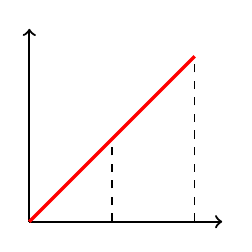
\begin{tikzpicture}[scale=0.7]
\draw[thick,->] (0,0)--(3.5,0);
\draw[thick,->] (0,0)--(0,3.5);
\draw[very thick, red] (0,0)--(3,3);
\draw[dashed] (3,0)--(3,3);
\draw[dashed] (1.5,0)--(1.5,1.5);
\end{tikzpicture}
\end{figure}

\section{Листинги}

В работах студентов кафедры <<Компьютерные технологии>> часто встречаются листинги. Листинги бывают
двух основных видов~--- исходный код и псевдокод. Первый оформляется с помощью окружения \texttt{lstlisting}
из пакета \texttt{listings}, который уже включается в стилевике и немного настроен. Пример Hello World на Java
приведен на листинге~\ref{lst1}. Пример большого листинга~--- в приложении (листинг~\ref{lstX}).

\begin{lstlisting}[float=!h,caption={Пример исходного кода на Java},label={lst1}]
public class HelloWorld {
    public static void main(String[] args) {
        System.out.println("Hello, world!");
    }
}
\end{lstlisting}

Псевдокод можно оформлять с помощью разных пакетов. В данном стилевике включается пакет \texttt{algorithmicx}.
Сам по себе он не генерирует флоатов, поэтому для них используется пакет \texttt{algorithm}.
Пример их совместного использования приведен на листинге~\ref{lst2}.

\begin{algorithm}[!h]
\caption{Пример псевдокода}\label{lst2}
\begin{algorithmic}
	\Function{IsPrime}{$N$}
		\For{$t \gets [2; \lfloor\sqrt{N}\rfloor]$}
			\If{$N \bmod t = 0$}
				\State\Return \textsc{false}
			\EndIf
		\EndFor
		\State\Return \textsc{true}
	\EndFunction
\end{algorithmic}
\end{algorithm}

Наконец, листинги из \texttt{listings} тоже можно подвешивать с помощью \texttt{algorithm},
пример на листинге~\ref{lst3}.

\begin{algorithm}[!h]
\caption{Исходный код и флоат \texttt{algorithm}}\label{lst3}
\begin{lstlisting}
public class HelloWorld {
    public static void main(String[] args) {
        System.out.println("Hello, world!");
    }
}
\end{lstlisting}
\end{algorithm}

\chapter{Проверка сквозной нумерации}

Листинг~\ref{lst4} должен иметь номер 4.

\begin{algorithm}[!h]
\caption{Исходный код и флоат \texttt{algorithm}}\label{lst4}
\begin{lstlisting}
public class HelloWorld {
    public static void main(String[] args) {
        System.out.println("Hello, world!");
    }
}
\end{lstlisting}
\end{algorithm}

Рисунок~\ref{fig2} должен иметь номер 2.

\begin{figure}[!h]
\caption{Пример рисунка}\label{fig2}
\centering
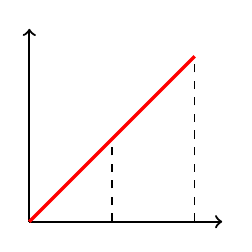
\begin{tikzpicture}[scale=0.7]
\draw[thick,->] (0,0)--(3.5,0);
\draw[thick,->] (0,0)--(0,3.5);
\draw[very thick, red] (0,0)--(3,3);
\draw[dashed] (3,0)--(3,3);
\draw[dashed] (1.5,0)--(1.5,1.5);
\end{tikzpicture}
\end{figure}

Таблица~\ref{tab3} должна иметь номер 3.

\begin{table}[!h]
\caption{Таблица умножения с помощью \texttt{tabularx} (фрагмент)}\label{tab3}
\centering
\begin{tabularx}{\textwidth}{|*{18}{>{\centering\arraybackslash}X|}}\hline
-- & 1 & 2 & 3 & 4 & 5 & 6 & 7 & 8 & 9 & 10 & 11 & 12 & 13 & 14 & 15 & 16 & 17 \\\hline
1  & 1 & 2 & 3 & 4 & 5 & 6 & 7 & 8 & 9 & 10 & 11 & 12 & 13 & 14 & 15 & 16 & 17 \\\hline
2  & 2 & 4 & 6 & 8 & 10 & 12 & 14 & 16 & 18 & 20 & 22 & 24 & 26 & 28 & 30 & 32 & 34 \\\hline
3  & 3 & 6 & 9 & 12 & 15 & 18 & 21 & 24 & 27 & 30 & 33 & 36 & 39 & 42 & 45 & 48 & 51 \\\hline
4  & 4 & 8 & 12 & 16 & 20 & 24 & 28 & 32 & 36 & 40 & 44 & 48 & 52 & 56 & 60 & 64 & 68 \\\hline
\end{tabularx}
\end{table}

\chapterconclusion

В конце каждой главы желательно делать выводы. Вывод по данной главе~--- нумерация работает корректно, ура!

%% Макрос для заключения. Совместим со старым стилевиком.
\startconclusionpage

В данном разделе размещается заключение.

\printmainbibliography

%% После этой команды chapter будет генерировать приложения, нумерованные русскими буквами.
%% \startappendices из старого стилевика будет делать то же самое
\appendix

\chapter{Пример приложения}\label{sec:app:1}

В приложениях рисунки, таблицы и другие подобные элементы нумеруются по приложениям с соответствующим префиксом. Проверим это.

Листинг~\ref{lst4:apx} должен иметь номер А.1.

\begin{algorithm}[!h]
\caption{Исходный код и флоат \texttt{algorithm}}\label{lst4:apx}
\begin{lstlisting}
public class HelloWorld {
    public static void main(String[] args) {
        System.out.println("Hello, world!");
    }
}
\end{lstlisting}
\end{algorithm}

Рисунок~\ref{fig2:apx} должен иметь номер A.1.

\begin{figure}[!h]
\caption{Пример рисунка}\label{fig2:apx}
\centering
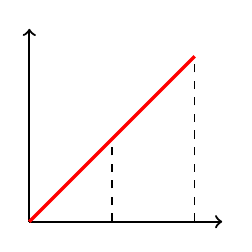
\begin{tikzpicture}[scale=0.7]
\draw[thick,->] (0,0)--(3.5,0);
\draw[thick,->] (0,0)--(0,3.5);
\draw[very thick, red] (0,0)--(3,3);
\draw[dashed] (3,0)--(3,3);
\draw[dashed] (1.5,0)--(1.5,1.5);
\end{tikzpicture}
\end{figure}

Таблица~\ref{tab3:apx} должна иметь номер A.1.

\begin{table}[!h]
\caption{Таблица умножения с помощью \texttt{tabularx} (фрагмент)}\label{tab3:apx}
\centering
\begin{tabularx}{\textwidth}{|*{18}{>{\centering\arraybackslash}X|}}\hline
-- & 1 & 2 & 3 & 4 & 5 & 6 & 7 & 8 & 9 & 10 & 11 & 12 & 13 & 14 & 15 & 16 & 17 \\\hline
1  & 1 & 2 & 3 & 4 & 5 & 6 & 7 & 8 & 9 & 10 & 11 & 12 & 13 & 14 & 15 & 16 & 17 \\\hline
2  & 2 & 4 & 6 & 8 & 10 & 12 & 14 & 16 & 18 & 20 & 22 & 24 & 26 & 28 & 30 & 32 & 34 \\\hline
3  & 3 & 6 & 9 & 12 & 15 & 18 & 21 & 24 & 27 & 30 & 33 & 36 & 39 & 42 & 45 & 48 & 51 \\\hline
4  & 4 & 8 & 12 & 16 & 20 & 24 & 28 & 32 & 36 & 40 & 44 & 48 & 52 & 56 & 60 & 64 & 68 \\\hline
\end{tabularx}
\end{table}

Заодно проверим нумерованные и ненумерованные перечисления. Ненумерованные:
\begin{itemize}
    \item пункт А;
    \item пункт Б;
    \item пункт В.
\end{itemize}

Нумерованные списки нескольких уровней:
\begin{enumerate}
    \item первый элемент;
    \item второй элемент с подэлементами:
    \begin{enumerate}
        \item первый подэлемент;
        \item второй подэлемент;
        \item третий подэлемент.
    \end{enumerate}
    \item третий элемент;
    \item четвертый элемент;
    \item пятый элемент;
    \item шестой элемент;
    \item седьмой элемент;
    \item восьмой элемент;
    \item девятый элемент;
    \item десятый элемент.
\end{enumerate}

\chapter{Еще один пример приложения с неимоверно длиннющим названием для тестирования переносов}\label{sec:app:2}

Проверим на примере таблиц, что нумерация в приложениях~--- по приложениям.
Таблица~\ref{tab3:apx2} должна иметь номер Б.1.

\begin{table}[!h]
\caption{Таблица умножения с помощью \texttt{tabularx} (фрагмент)}\label{tab3:apx2}
\centering
\begin{tabularx}{\textwidth}{|*{18}{>{\centering\arraybackslash}X|}}\hline
-- & 1 & 2 & 3 & 4 & 5 & 6 & 7 & 8 & 9 & 10 & 11 & 12 & 13 & 14 & 15 & 16 & 17 \\\hline
1  & 1 & 2 & 3 & 4 & 5 & 6 & 7 & 8 & 9 & 10 & 11 & 12 & 13 & 14 & 15 & 16 & 17 \\\hline
2  & 2 & 4 & 6 & 8 & 10 & 12 & 14 & 16 & 18 & 20 & 22 & 24 & 26 & 28 & 30 & 32 & 34 \\\hline
3  & 3 & 6 & 9 & 12 & 15 & 18 & 21 & 24 & 27 & 30 & 33 & 36 & 39 & 42 & 45 & 48 & 51 \\\hline
4  & 4 & 8 & 12 & 16 & 20 & 24 & 28 & 32 & 36 & 40 & 44 & 48 & 52 & 56 & 60 & 64 & 68 \\\hline
\end{tabularx}
\end{table}

\chapter{Пример огромного листинга}

\begin{lstlisting}[caption={Пример большого листинга},label={lstX}]
import java.util.*;

public class Example {
    static int[] restoreOutgoing(int[] g, int[] outgoing,
                                 int vertex, int mask) {
        int[] rv = new int[1 + Integer.bitCount(mask)];
        int n = g.length;
        int current = rv.length - 1;
        while (true) {
            rv[current] = vertex;
            if (current == 0) {
                if (vertex != 0) {
                    throw new AssertionError();
                }
                return rv;
            }
            mask ^= 1 << (vertex - 1);
            int prevMask = outgoing[mask] & g[vertex];
            if (prevMask == 0) {
                throw new AssertionError();
            }
            vertex = Integer.numberOfTrailingZeros(prevMask);
            --current;
        }
    }

    static int[] restoreIncoming(int[] g, int[] incoming,
                                 int vertex, int mask) {
        int[] rv = new int[1 + Integer.bitCount(mask)];
        int n = g.length;
        int current = 0;
        while (true) {
            rv[current] = vertex;
            if (current == rv.length - 1) {
                if (vertex != 0) {
                    throw new AssertionError();
                }
                return rv;
            }
            mask ^= 1 << (vertex - 1);
            int nextMask = incoming[mask] & g[vertex];
            if (nextMask == 0) {
                throw new AssertionError();
            }
            vertex = Integer.numberOfTrailingZeros(nextMask);
            ++current;
        }
    }
}
\end{lstlisting}

\end{document}
